% $Id: CONTENT.tex 12319 2010-09-24 12:26:35Z alexandra $
% Local Variables:
% ispell-check-comments: nil
% Local IspellDict: american
% End:
% --------------------------------------------------------
% User documentation
% copyright by BREDEX GmbH 2004
% --------------------------------------------------------
\gdcases{} are the ''building blocks'' (keywords) in \jb{}. They can: 
\begin{itemize}

\item contain other (referenced) \gdcases{} \bxpref{addtestcase}
\item contain \gdsteps{} \bxpref{specsteps}
\item be used in \gdsuites{} \bxpref{addtestsuite}
\item be used as \gdehandlers{} \bxpref{customizedehandler}
\end{itemize}

\subsection{Creating \gdcases{}}
\gdhelpid{testcaseNewContextId}{New Test Case Dialog}
\gdhelpid{guidancerSpecTestCaseEditorContextId}{Test Case Editor}
\gdhelpid{testSpecificationViewContextId}{Test Case Browser}
\label{TasksCreateTC}
% $Id: specifyTestCases.tex 8144 2009-04-03 15:27:38Z alexandra $
% Local Variables:
% ispell-check-comments: nil
% Local IspellDict: american
% End:
% --------------------------------------------------------
% User documentation
% copyright by BREDEX GmbH 2004
% -------------------------------------------------------
\index{New!Test Case}
\index{Test Case!New}

Most of the time spent writing tests will involve creating and editing \gdcases{}. 

To create a \gdcase{}, you must have created or opened a \gdproject{} \bxpref{WorkingWithProjects}. 

The \gdtestcasebrowser{} must also be visible. If it is not visible, change to the specification perspective and select:\\
\bxmenu{Window}{Show View}{Test Case Browser}.

\begin{enumerate}
\item Create a \gdcase{} by using the context-sensitive menu in the \gdtestcasebrowser{}:\\
\bxmenu{New}{New \gdcase{}}{}.
\bxtipp{You can also create \gdcases{} with a double-click on the \bxcaption{\gdcases{}:} root entry or on a category in the \gdtestcasebrowser{}.}

\item A dialog to name the \gdcase{} will appear (\bxfigref{newtestcasedialog}). Because \jb{} is keyword-driven, it is important to name \gdcases{} meaningfully --  you will be able to read your tests easily and quickly choose which \gdcase{} you need  \bxpref{BPTestCaseNames}. 

\begin{figure}[h]
\begin{center}
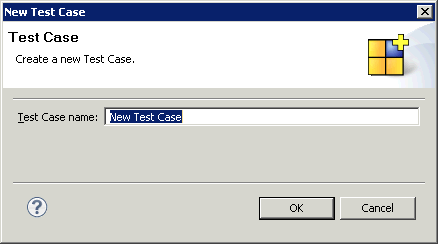
\includegraphics[width=12.5cm]{Tasks/Testcases/PS/newtestcasedialog}
\caption{New \gdcase{} Dialog}
\label{newtestcasedialog}
\end{center}
\end{figure} 

\item Click \bxcaption{OK}. 
\item This creates a new \gdcase{} with that name in the \gdtestcasebrowser{} \bxfigref{newtestcaseinbrowser}.

\begin{figure}[h]
\begin{center}
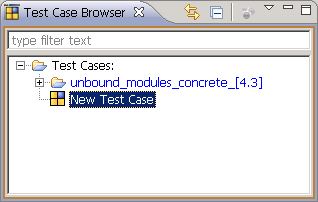
\includegraphics{Tasks/Testcases/PS/newtestcaseinbrowser}
\caption{\gdcase{} in \gdtestcasebrowser{}}
\label{newtestcaseinbrowser}
\end{center}
\end{figure} 

\end{enumerate}

\bxtipp{See the Best Practices section for information on how to best structure your \gdcases{} and tests \bxpref{BPKeywordDesign}.}
\textbf{Next steps}\\
The next step is to:
\begin{itemize}
\item Add \gdcases{} from the library of \gdcases{} to this \gdcase{}\bxpref{usingtemplate}. 

%\item Add \gdsteps{} \bxpref{specsteps} to it
%\item Add other \gdcases{} to it \bxpref{addtestcase}
%\bxtipp{Remember, you can also add \gdcases{} from the \gdcase{} library \bxpref{usingtemplate}. This will make test creation easier and quicker.}
\end{itemize}

You can also:
\begin{itemize} 
\item Reuse this \gdcase{} to form other \gdcases{}  \bxpref{addtestcase}
\item Edit its content in the \gdtestcaseeditor{} \bxpref{edittestcase}
\item Add this \gdcase{} to a \gdsuite{} to be executed \bxpref{addtestsuite}
\item Use this \gdcase{} as an \gdehandler \bxpref{customizedehandler}. 
\end{itemize}















\subsection{Creating tests from the library of pre-defined \gdcases{}}
\gdhelpid{guidancerSpecTestCaseEditorContextId}{Test Case Editor}
\gdhelpid{testCaseAddExistingContextId}{Existing Test Case Dialog}
\gdhelpid{testSpecificationViewContextId}{Test Case Browser}
\label{usingtemplate}
\index{Test Case!Library}
\index{Library of Test Cases}

Everything you need to create tests is already available for you in each \gdproject{}. The library of \gdcases{} which appears automatically in each new \gdproject{} contains all the actions supported by \app{} as well as some examples of more complex keywords. For general information about the library, read the section later on \bxpref{LibraryInformation}. To learn how to use the library to create tests, read the next section \bxpref{UseLibrary}. 


\subsubsection{Using the library to create tests}
\label{UseLibrary}
Creating tests with \app{} is really just a matter of:
\begin{itemize}
\item Deciding how to structure your tests (i.e. what keywords to create and how to combine them \bxpref{KeywordDesign}).
\item Choosing the \gdcases{} from the library (or from your own set of \gdcases{}) that you need to create these keywords. 
\end{itemize}

To use the \gdcases{} from the library, you will first need to create a \gdcase{} of your own \bxpref{TasksCreateTC}. 

\begin{enumerate}
\item Open the \gdtestcaseeditor{} by double-clicking on the \gdcase{} you want to edit in the \gdtestcasebrowser{}. 
\item In the \gdtestcasebrowser{}, browse to a \gdcase{} that you want to add. For help on finding your way around the library, see the later section \bxpref{UnderstandingLibrary}. 
\item You can add the \gdcase{} by dragging and dropping from the \gdtestcasebrowser{} to the \gdtestcaseeditor{} or you can right click on the \gdcase{} in the \gdtestcaseeditor{} and select:\\
\bxmenu{Reference Existing \gdcase{}}{}\\
to see a list of all \gdcases{} that you can add to this \gdcase{}. 

\bxtipp{You can filter in this dialog using the field at the top. Use star \bxshell{*} as a wild card.}

\bxtipp{You can open the dialog to reference an existing \gdcase{} by pressing \bxkey{Enter} on a \gdcase{} in the \gdtestcaseeditor{}.}

\item Once you have added the \gdcase{}, you will need to enter a component name in the \gdcompnamesview{} \bxpref{TasksReassignCompName} and you will need to enter data for the \gdcase{} in the \gdpropview{} \bxpref{WorkingWithData}. 
\bxtipp{See the Best Practices section for information on how to best structure your \gdcases{} and tests \bxpref{BPKeywordDesign}.}
\end{enumerate}


\subsubsection{Information about the library}
\label{LibraryInformation}
\begin{enumerate}
\item \app{} lets you use a  highly reusable library of \gdcases{} to specify tests. 
\item The \gdprojects{} containing the \gdcase{} libraries are located under:\\
\bxname{examples/testcaseLibrary}.

\item The \gdprojects{} available are:
\begin{itemize}
\item unbound\_modules\_concrete
\item unbound\_modules\_web
\item unbound\_modules\_swt
\item unbound\_modules\_rcp
\end{itemize}

\item These \gdprojects{} contain reusable \gdcases{} which have been created in advance so you do not have to specify them yourself.
\bxtipp{Refer to the chapter on Components, Actions, and Parameters
(\bxextref{\gdrefman}{ref,actparam}) for information on components, the
actions they support, and their parameters.}
\item The library is split into categories of \bxname{actions} on components. To select something in your \gdaut{}, open the \bxname{select} category and then open the category for the type of component you want to select something from. 

\bxtipp{The names for these \gdcases{} all begin with \bxcaption{ub}. This means that they are \bxname{unbound} -- they are not in any way dependent on an \gdaut{}. }
\item Each \gdcase{} in the library contains one \gdstep{} which corresponds to the action in the \gdcase{} name. The component name is a placeholder, and the parameters have been referenced so that you can enter your own data. 

\bxtipp{The unbound modules \gdprojects{} which correspond to your chosen \gdproject{} toolkit are automatically imported into the \gddb{} and reused in your \gdproject{}.}
 

\bxwarn{We do not recommend making changes to the installed unbound module \gdprojects{}, for compatibility reasons. If you have \gdcases{} you want to reuse in other \gdprojects{}, we advise creating your own library \gdproject{}.}


\end{enumerate}

\subsubsection{Tips and tricks for using the \gdcase{} library}
\label{UnderstandingLibrary}
The \gdcases{} in the library are organised into actions. In the \bxname{basic} category, you will find the various actions offered by \app{}. The \bxname{complex} category contains some example keywords which are built up of more than one \gdcase{}. 

When specifying your tests, you need to find and choose which actions you will need. This takes some practice, but there are some hints which can help you:

\textbf{High-Level Actions}\\
\app{} executes \bxname{high-level} actions. This means that if you want to select something from a menu using the menupath, for example, you need to look in the category:\\
\bxname{Actions (basic)/Select/Menu Bar}\\
and select the \gdcase{}:\\
\bxname{ub\_mbr\_selectEntry\_byTextpath}\\
The \gdcase{} finds the menu, opens it, and clicks the item you specify. \\

\textbf{Abstract components}\\
There are some actions which are executable on many different components. Clicks, for example can be executed on pratically all components in the interface. You can also check text on labels, combo boxes and text fields. Obviously, it makes sense to specify your \gdcases{} as abstractly as possible so that they can be reused in more places. This helps keep the maintenance low later. 

You will notice in the library that there is no \bxname{Button} category under the \bxname{Click} category. Instead, you will find various click actions specified for \bxname{Graphics Component (grc)}. This is because all components which support clicks belong to the \bxname{Graphics Component} group. 

In the same way, you will find the category \bxname{Check/Component with Text}. You can use the check actions from this category to check text on any component with text -- buttons, text fields, combo boxes, labels. \\

\textbf{Parameters}\\
Different actions require different data. Some \gdcases{} in the library have been pre-configured with data to make test specification easier (look in the category \bxname{Input via Keyboard/Application/Key Combination} for a long list). 

Some actions let you choose whether you want to enter data using an \bxname{indexpath} or a \bxname{textpath}. We recommend using the textpath so that you are not dependent on the order of e.g. menu entries or tabbed panes. 

To make text-based parameters more robust, \app{} often lets you choose an \bxname{operator}. You can choose between \bxname{equals, matches, simple match, not equals}. Using matches lets you use regular expressions so that you don't have to hard-code the whole text parameter. 






\subsection{Opening \gdcases{}}
\gdhelpid{guidancerSpecTestCaseEditorContextId}{Test Case Editor}
\gdhelpid{testCaseOpenExistingContextId}{Open Existing Test Case}
You can open an existing \gdcase{} without having to select it from the \gdtestcasebrowser{} using the \bxname{Open Test Case} dialog. 

\begin{enumerate}
\item  This dialog can be opened using the shortcut \bxkey{Ctrl+Shift+T} or from the menu:\\
\bxmenu{Edit}{Open Test Case}{}
\item In the dialog, you can search for a \gdcase{} or \gdcases{} in the tree or using the filter \bxpref{TasksFilters}. 
\item Select the \gdcases{} you want to add, and clic \bxcaption{OK}.
\item The selected \gdcases{} will be opened in indidivual \gdcase{} editors. 
\end{enumerate}

\bxtipp{You can use this option to open a \gdcase{} even if a filter is active in the \gdtestcasebrowser{}.}


\subsection{Deleting \gdcases}
\gdhelpid{testSpecificationViewContextId}{Test Case Browser}
\index{Component!Names!Delete}
\index{Delete!Component Names}

When you reassign component names in the \gdcompnamesview{}, you automatically create new component names if the name you enter did not previously exist in the \gdproject{}. 

Larger \gdprojects{} can often end up with a number of component names that are no longer used. You can see and delete these names in the \gdcompnamebrowser{}. 
The names in the \bxname{Unused Component Names} category are not used anywhere in this \gdproject{} -- they are not present in any \gdcases{} and they have not been mapped to any technical names from the \gdaut{} in the \gdomeditor{} (\bxfigref{}). 

\begin{figure}[h]
\begin{center}
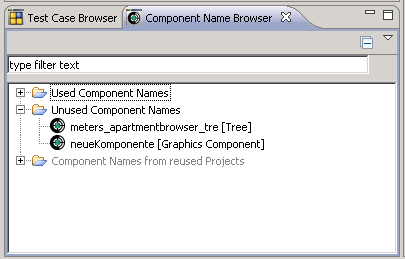
\includegraphics{Tasks/Compnames/PS/compnamebrowser}
\caption{The \gdcompnamebrowser{}}
\label{compnamebrowser}
\end{center}
\end{figure} 

To delete unused component names, select the name you want to delete and select:\\
\bxmenu{Delete}{}{}\\
from the context-menu. 



\subsection{Editing \gdcases{}: renaming, adding comments, deleting items}
\gdhelpid{testSpecificationViewContextId}{Test Case Browser}
\gdhelpid{guidancerSpecTestCaseEditorContextId}{Test Case Editor}
%% \gdhelpid{testSuiteEditorContextId}{Test Suite Editor}
%% \gdhelpid{testExecViewContextId}{Test Suite Browser}
\label{edittestcase}
\index{Test Suite!Configuration}
\index{Configuration!Test Suite}
\index{Event Handler!Error Types}
\index{Error Types}
\index{Action Error}
\index{Component not found}
\index{Check failed}
\index{Configuration error}
\index{Reentry Properties}
\index{Event Handler!Reentry Properties}
\index{Break}
\index{Continue}
\index{Return}
\index{Pause}
\index{Exit}
\index{Default Event Handler}
\index{Event Handler!Default}
\index{AUT ID}
\label{confsuite}

To configure a \gdsuite{}, you must first create one \bxpref{TSeditor}.

\bxtipp{If you are editing the \gdsuite{}, the working language (which is specified via the globe button on the toolbar) must be set to a language supported by the chosen \gdaut{} for the \gdsuite{}. Otherwise the \gdsuite{} will be uneditable. }

\begin{enumerate}
\item Open the \gdtestsuiteeditor{} by double-clicking on the \gdsuite{} you want to configure. 
\item In the \gdpropview{}, you can:
\begin{enumerate}
\item Change the \gdsuite{} name by entering a new name in the \bxname{\gdsuite{} name} field.  
\item Add a comment to the \gdsuite{} \bxpref{TasksEditorAddComment}. 
\item Enter a value in the \bxname{step delay} field. The step delay is the time left between each \gdstep{} during test execution. The default is 0 milliseconds \bxpref{TasksExecSpeed}.
\item Enter a Task ID to link this \gdsuite{} to a task in an external system \bxpref{TasksALMAddTask}.
\item Set whether this \gdsuite{} should be relevant or not. If a \gdsuite{} is marked as non-relevant, test results for ths \gdsuite{} are created but are not exported with the \gdproject{}, are not considered for any BIRT reports \bxpref{TasksBIRT} and do not save details to be reported to external ALM repositories \bxpref{TasksALMReport}. 
\item Select the \gdaut{} for this \gdsuite{}. To be able to select an \gdaut{} (and object map, and execute your test) you must have added at least one \gdaut{} to the \gdproject{} \bxpref{Defineaut}.
\bxtipp{You don't have to choose an \gdaut{} for a \gdsuite{} as soon as you have created it, but you will have to choose one before object mapping, for example.}

\item Choose a default reentry type for each of the four error types  from the combo-boxes. 

\gdehandlers{} are \gdcases{} used to deal with errors during test execution. When an error occurs, the current \gdcase{} is searched for an \gdehandler{} for that error type. If none is found, the parent \gdcase{} is searched, and so on. If no \gdehandler{} for the test is found, then a default \gdehandler{} (specified in the \gdsuite{} properties)is activated.  

As a general rule, you should avoid default \gdehandlers{} being executed.
See the sections on \gdehandlers{} for information on the event types \bxpref{eventtype}, reentry types \bxpref{reentrytype} and creating your own \gdehandlers{}.
\item Save the changes in the \gdtestsuiteeditor{}.
\end{enumerate}
\end{enumerate}


\subsection{Adding existing \gdcases{} to a \gdcase{}}
\gdhelpid{guidancerSpecTestCaseEditorContextId}{Test Case Editor}
\gdhelpid{testCaseAddExistingContextId}{Existing Test Case Dialog}
\label{addtestcase}
%% \index{Add!Test Cases}
%% \index{Test Case!Add}
%% For specific information on adding \gdcases{} from the library, see the previous section \bxpref{usingtemplate}. 
%% \begin{enumerate}
%% \item Open the \gdtestcaseeditor{} by double-clicking on the \gdcase{} you want to edit in the \gdtestcasebrowser{}. 
%% \item Select a \gdcase{} via the context-sensitive menu in the \gdtestcasebrowser{} by selecting:
%% \bxmenu{Reference Existing \gdcase{}}{}{}\\

%% \bxtipp{You can also add \gdcases{} by dragging them from the \gdtestcasebrowser{} or by pressing \bxkey{ENTER} on a selected \gdcase{} in the \gdtestcaseeditor{}. You can filter in the \gdtestcasebrowser{} using the field at the top. Use star \bxshell{*} as a wild card.}

%% \item Choose a \gdcase{} or \gdcases{} to add from the dialog which appears (\bxfigref{referencetestcasedialog}).

%% \bxtipp{You can filter in this dialog using the field at the top. Use star \bxshell{*} as a wild card.}

%% \begin{figure}[h]
%% \begin{center}
%% 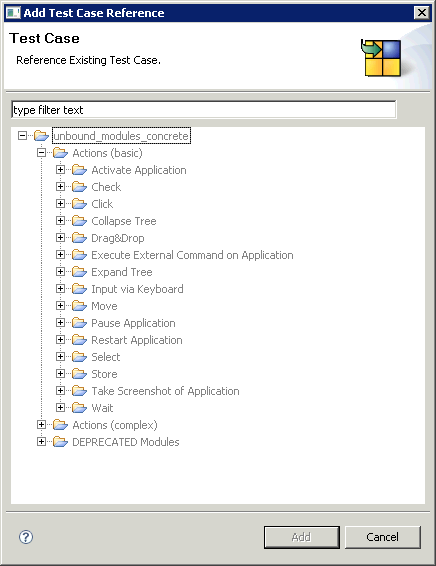
\includegraphics{Tasks/Testcases/PS/referencetestcasedialog}
%% \caption{Add \gdcase{} reference dialog}
%% \label{referencetestcasedialog}
%% \end{center}
%% \end{figure} 

%% \item Click \bxcaption{OK}. 

%% \item The \gdcase{} or \gdcases{} you selected appear(s) in the \gdtestcaseeditor{}. They are marked with a small arrow to show that they are reused (referenced) here. The name of the \gdcase{} is contained in angled brackets (\bxshell{< >}) to show that it is the same name that you used when you specified the \gdcase{}. 
%% \item Save the changes in the editor.
%% \end{enumerate}

%% \bxwarn{You can't add a \gdcase{} which would cause an infinite loop.}


\subsection{Adding new \gdcases{} to a \gdcase{}}
\gdhelpid{dialogTestcaseAddNewContextId}{Add New Test Case Dialog}
\gdhelpid{dialogTestcaseInsertNewContextId}{Insert New Test Case Dialog}
\begin{enumerate}
\item Open the \gdtestcaseeditor{} by double-clicking on the \gdcase{} you want to edit in the \gdtestcasebrowser{}. 
\item From the context-sensitive menu, select:
\bxmenu{Add}{New \gdcase{}}{}\\
(This places the \gdcase{} after any other items in the \gdtestcaseeditor{}.)
or\\
\bxmenu{Insert}{New \gdcase{}}{}\\
(This places the \gdcase{} above the currently selected item in the \gdtestcaseeditor{}.)

\item In the dialog that appears, enter a meaningful name for the new \gdcase{}. 
\item Click \bxcaption{OK}. 
\item The \gdcase{} appears in the \gdtestcaseeditor{} in the parent  \gdcase{} and also appears in the \gdtestcasebrowser{}.  The \gdcase{} is  marked with a small arrow to show that it is  reused here. The name of the \gdcase{} is contained in angled brackets (\bxshell{< >}) to show that it is the same name that you used when you specified the \gdcase{}. 
\item Save the changes in the editor.
\end{enumerate}


\subsection{Categories for \gdcases{}}
\gdhelpid{testSpecificationViewContextId}{Test Case Browser}
\gdhelpid{dialogNewCategoryContextId}{New Category Dialog}
\label{TasksTCCats}
% $Id: Categories.tex 12283 2010-09-23 10:34:38Z alexandra $
% Local Variables:
% ispell-check-comments: nil
% Local IspellDict: american
% End:
% --------------------------------------------------------
% User documentation
% copyright by BREDEX GmbH 2005
% --------------------------------------------------------
% this command can be inserted multiple times
%\gdhelpid{}
% 
%\begin{gddescription}
%\end{gddescription}
%
%\begin{gdlist}
% use the \item command for single steps
%\end{gdlist}
% change <PATH> to the same directory, file is located in
% change <FILE> to the same filename you are editing
%\bxinput{<PATH>/Links/<FILE>}
%
% other usefull commands are
%   \bxtipp{}        to create a hint
%   \bxwarn{}        to describe a warning
\index{Categories!Test Cases}
\index{Test Case!Categories}
Categories let you  group \gdcases{} together in the \gdtestcasebrowser{}. 

\textbf{Creating a category:}
\begin{enumerate}
\item In the \gdtestcasebrowser{}, select:\\
\bxmenu{New}{Category}{} from the context-sensitive menu. 
\item Name the category when prompted.
\item You can add \gdcases{} to this category using drag-and-drop.  
\item You can also nest categories in other categories. 
\item You can do this either by dragging and dropping a category into another category, or by right-clicking in an already present category and choosing the option to create a new category. 
\bxtipp{For best practices on how to use categories in the \gdtestcasebrowser{}, see the section on Best Practices \bxpref{BPCategories}}
\end{enumerate}

\textbf{Creating \gdcases{} in a category:}
\begin{enumerate}
\item In the \gdtestcasebrowser{}, select the category in which you want to create the \gdcase{} with a single-click. 
\item Create a \gdcase{} via the context-sensitive menu \bxpref{TasksCreateTC}.
\item You can also simply double-click on the category in which you want to create the \gdcase{}. 
\end{enumerate}




\subsection{Commenting out \gdcases{} and \gdsteps{}}
\gdhelpid{guidancerSpecTestCaseEditorContextId}{Test Case Editor}
\gdhelpid{testSuiteEditorContextId}{Test Suite Editor}
In the \gdtestcaseeditor{} and the \gdtestsuiteeditor{}, you can deactivate and reactivate \gdcases{} and \gdsteps{}. 

\begin{enumerate}
\item Select the \gdsteps{} or \gdcases{} you want to deactivate and select:\\
\bxmenu{Set as active / inactive}{}{}\\
from the context menu.
\bxtipp{You can also use \bxkey{ctrl+7} to toggle the items as active or inactive.}
\item The items you selected will be set as inactive. They are shown with green text and the sign \verb+//+ before the \gdcase{} or \gdstep{} name.
\item Any inactive items are not considered in \gdsuite{} validation, nor are they executed during a test run. 
\item You can reactivate the items by selecting:\\
\bxmenu{Set as active / inactive}{}{}\\
from the context menu.
\end{enumerate}


\subsection{Extracting a new \gdcase{} (refactoring)}
\gdhelpid{guidancerSpecTestCaseEditorContextId}{Test Case Editor}
\gdhelpid{testSuiteEditorContextId}{Test Suite Editor}
\label{extract}
% $Id: Extracting.tex 7785 2009-02-03 16:16:16Z alexandra $
% Local Variables:
% ispell-check-comments: nil
% Local IspellDict: american
% End:
% --------------------------------------------------------
% User documentation
% copyright by BREDEX GmbH 2005
% --------------------------------------------------------
% this command can be inserted multiple times
%\gdhelpid{}
% 
%\begin{gddescription}
%\end{gddescription}
%
%\begin{gdlist}
% use the \item command for single steps
%\end{gdlist}
% change <PATH> to the same directory, file is located in
% change <FILE> to the same filename you are editing
%\bxinput{<PATH>/Links/<FILE>}
%
% other usefull commands are
%   \bxtipp{}        to create a hint
%   \bxwarn{}        to describe a warning

\index{Test Case!Extracting}
\index{Extracting!Test Case}
\gd{} lets you \bxname{extract} \gdcases{} from other \gdcases{}. This lets you create keywords even after you have started specifying. 

\begin{enumerate}
\item Open the \gdtestcaseeditor{} by double-clicking on the \gdcase{} you want to edit in the \gdtestcasebrowser{}. 
\item Select the \gdcases{} you want to extract by single-clicking them. Use 
  \bxkey{Ctrl} to select more than one item. 
\item Right-click in the editor and  select: \\
\bxmenu{Refactor}{Extract Test Case}{}.
\item When prompted, enter a name for the new \gdcase{}. 
\item The \gdcases{} you selected will be extracted into this new \gdcase{}. 
\item The extracted \gdcase{} appears as a reused \gdcase{} in the current editor. It is marked with a small arrow to show that it is reused, and the \gdcase{} name is in angled brackets (\bxshell{< >}) to show that it is the same as the specification name. 
\item The \gdcase{} you just created is also visible in the \gdtestcasebrowser{}. 
\end{enumerate}
\bxtipp{Use this feature when you realize that you are planning on reusing one or more \gdcases{} for the same or a similar action again. You will save yourself time in test creation and maintenance.}



\subsection{Reverting changes in an editor}
\gdhelpid{guidancerSpecTestCaseEditorContextId}{Test Case Editor}
\gdhelpid{testSuiteEditorContextId}{Test Suite Editor}
\index{Revert changes}
You can revert an editor you are working in to the state of the last save.
\begin{enumerate}
\item In the editor you are in, right-click and select:\\
\bxmenu{Revert changes}{}{}\\
from the context sensitive menu. 
\item Confirm that you want to revert the changes when prompted. 
\item The editor will be reverted. Any changes you have made since the last save will be lost. 
\end{enumerate}


\subsection{Moving \gdcases{} to external \gdprojects{}}
\gdhelpid{testCaseMoveExternalContextId}{Move Test Cases to an External Project}
\gdhelpid{testSpecificationViewContextId}{Test Case Browser}
\label{movetoexternal}
I

If you are reusing a \gdproject{} or \gdprojects{} in your currently opened \gdproject{} \bxpref{reuseproject}, you can move \gdcases{} you create to these reused \gdprojects{} to make them a part of that \gdproject{}. 

This lets you add useful \gdcases{} to external libraries to be reused in other \gdprojects{}. 


\begin{enumerate}
\item In the \gdtestcasebrowser{}, select the \gdcase{}, \gdcases{} or categories you want to move to an external \gdproject{} that you are currently reusing in the open \gdproject{}. 
\item Right click on the selected items and select:\\
\bxmenu{Move to external Project}{}{}\\
from the context-sensitive menu. 
\item From the dialog which appears, select which reused \gdproject{} to move them to. 
\item The items you selected will appear in the grayed-out category of the reused \gdproject{} you selected and will disappear from their original place. 
\item The structure of your \gdproject{} stays the same -- the moved \gdcases{} are not deleted from places where you have reused them, for example. 
\end{enumerate}
\bxwarn{If you move \gdcases{} containing referenced \gdcases{} from other \gdprojects{}, make sure that the \gdproject{} the \gdcases{} are dependent on is also reused in your external \gdproject{}.}



\subsection{Working with tasks and repositories: Mylyn and \jb{}}
\gdhelpid{testSpecificationViewContextId}{Test Case Browser}
\gd{} is integrated with the Mylyn \gdproject{} to support task- and context-based work with your tests. 

Mylyn lets you:
\begin{itemize}
\item Reduce the amount of \gdcases{} and \gdsuites{} you can see in your \gdproject{} so that you can focus on a task. 
\item Switch between tasks, recreating the context (visible \gdcases{}, open editors) that you had for each task.
\item Connect to repositories such as Eclipse, TRAC etc. to manage tasks and tickets within the whole team. 
\end{itemize}

The Mylyn online help is included in \gd{}. 

Select:\\
 \bxmenu{Help}{Help Contents}{}\\
in the \gd{} client to see the Mylyn help. 

